%%%%%%%%%%%%%%%%%%%%%%%%%%%%%%%%%%%%%%%%%
% Beamer Presentation
% LaTeX Template
% Version 1.0 (10/11/12)
%
% This template has been downloaded from:
% http://www.LaTeXTemplates.com
%
% License:
% CC BY-NC-SA 3.0 (http://creativecommons.org/licenses/by-nc-sa/3.0/)
%
%%%%%%%%%%%%%%%%%%%%%%%%%%%%%%%%%%%%%%%%%

%----------------------------------------------------------------------------------------
%	PACKAGES AND THEMES
%----------------------------------------------------------------------------------------

\documentclass{beamer}

\mode<presentation> {

% The Beamer class comes with a number of default slide themes
% which change the colors and layouts of slides. Below this is a list
% of all the themes, uncomment each in turn to see what they look like.

%\usetheme{default}
%\usetheme{AnnArbor}
%\usetheme{Antibes}
%\usetheme{Bergen}
%\usetheme{Berkeley}
%\usetheme{Berlin}
%\usetheme{Boadilla}
%\usetheme{CambridgeUS}
%\usetheme{Copenhagen}
%\usetheme{Darmstadt}
%\usetheme{Dresden}
%\usetheme{Frankfurt}
%\usetheme{Goettingen}
%\usetheme{Hannover}
%\usetheme{Ilmenau}
%\usetheme{JuanLesPins}
%\usetheme{Luebeck}
\usetheme{Madrid}
%\usetheme{Malmoe}
%\usetheme{Marburg}
%\usetheme{Montpellier}
%\usetheme{PaloAlto}
%\usetheme{Pittsburgh}
%\usetheme{Rochester}
%\usetheme{Singapore}
%\usetheme{Szeged}
%\usetheme{Warsaw}

% As well as themes, the Beamer class has a number of color themes
% for any slide theme. Uncomment each of these in turn to see how it
% changes the colors of your current slide theme.

%\usecolortheme{albatross}
%\usecolortheme{beaver}
%\usecolortheme{beetle}
%\usecolortheme{crane}
%\usecolortheme{dolphin}
%\usecolortheme{dove}
%\usecolortheme{fly}
%\usecolortheme{lily}
%\usecolortheme{orchid}
%\usecolortheme{rose}
%\usecolortheme{seagull}
%\usecolortheme{seahorse}
%\usecolortheme{whale}
%\usecolortheme{wolverine}

%\setbeamertemplate{footline} % To remove the footer line in all slides uncomment this line
%\setbeamertemplate{footline}[page number] % To replace the footer line in all slides with a simple slide count uncomment this line

%\setbeamertemplate{navigation symbols}{} % To remove the navigation symbols from the bottom of all slides uncomment this line
}

\usepackage{graphicx} % Allows including images
\usepackage{booktabs} % Allows the use of \toprule, \midrule and \bottomrule in tables

%----------------------------------------------------------------------------------------
%	TITLE PAGE
%----------------------------------------------------------------------------------------

\title[Domotic Room Server]{Domotic Room Server} % The short title appears at the bottom of every slide, the full title is only on the title page

\author{Benini - Casadei - Benedetti} % Your name
\institute[Unibo] % Your institution as it will appear on the bottom of every slide, may be shorthand to save space
{
University of Bologna \\ % Your institution for the title page
\medskip
\textit{enrico.benini5@studio.unibo.it} % Your email address
\textit{nicola.casadei4@studio.unibo.it} % Your email address
\textit{marco.benedetti7@studio.unibo.it} % Your email address
}
\date{\today} % Date, can be changed to a custom date

%\setlength{\abovecaptionskip}{-2ex}
\setlength{\belowcaptionskip}{-2ex}

\begin{document}

\begin{frame}
\titlepage % Print the title page as the first slide
\end{frame}

\begin{frame}
\frametitle{Overview} % Table of contents slide, comment this block out to remove it
\tableofcontents % Throughout your presentation, if you choose to use \section{} and \subsection{} commands, these will automatically be printed on this slide as an overview of your presentation
\end{frame}

%----------------------------------------------------------------------------------------
%	PRESENTATION SLIDES
%----------------------------------------------------------------------------------------

%------------------------------------------------
\section{Domain Analysis} % Sections can be created in order to organize your presentation into discrete blocks, all sections and subsections are automatically printed in the table of contents as an overview of the talk
%------------------------------------------------

\subsection{Use Cases} % A subsection can be created just before a set of slides with a common theme to further break down your presentation into chunks

\begin{frame}
  \frametitle{Use Cases}
  \begin{center}
    Utilizzo principale della parte server.
   \end{center}
   \begin{figure}
     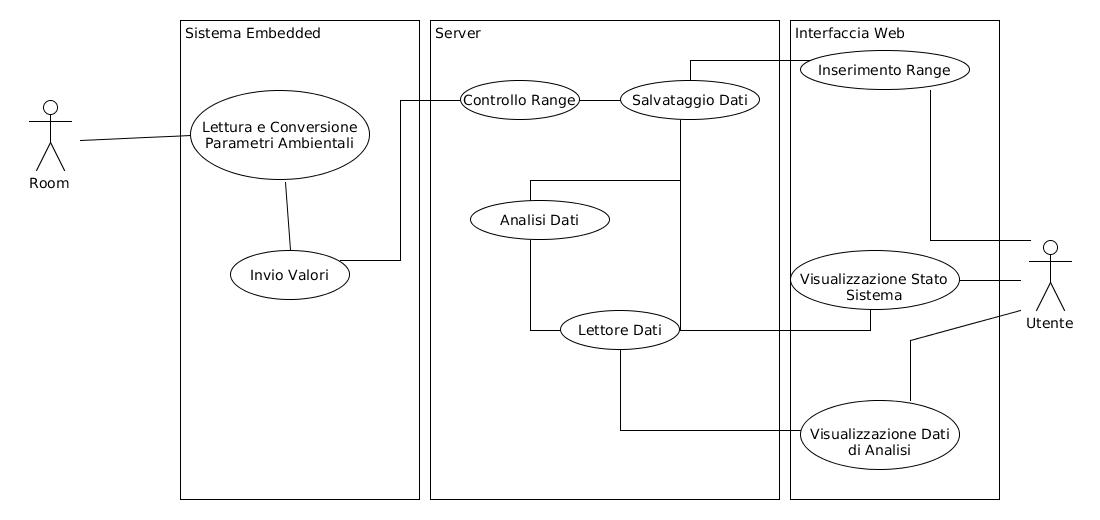
\includegraphics[width=0.8\linewidth]{../../Docs/ProjectReport/Figures/UseCases.jpg}
   \end{figure}
\end{frame}

%------------------------------------------------

\subsection{Domain Model}

\begin{frame}
  \frametitle{Domain Model - Structures}
  Entit\'a principali riguardanti il dominio applicativo
  \begin{itemize}
    \item Sensori: coloro che inviano i dati al server.
    \item Ranges: Intervalli su cui controllare la validit\'a  dei dati raccolti.
  \end{itemize}
  Entit\'a dai requsiti non funzionali
  \begin{itemize}
    \item PersistenceStore: Dove salvare i dati.
    \item Analizer: computa analisi sui dati.
  \end{itemize}
\end{frame}

\begin{frame}
  \frametitle{Domain Model - Interaction and Behaviour}
  \begin{columns}[c] % The "c" option specifies centered vertical alignment while the "t" option is used for top vertical alignment
    \column{.45\textwidth} % Left column and width
      Prime considerazioni riguardo l'interazione
    \begin{itemize}
      \item \textit{Polling:} come metodo per ottenere dati dai sensori.
      \item \textit{Procedure Call:} Viene invocata dall'estrerno una funzionalit\'a del sistema.
    \end{itemize}
    \column{.5\textwidth} % Right column and width
      Prime considerazioni riguardo il comportamento
    \begin{itemize}
      \item \textit{Wait:} Attesa dell'arrivo di una richiesta.
      \item \textit{Compute:} Viene effettuata una computazione sulla base della richiesta
      \item \textit{Output:} Viene mostrato il risultato.
    \end{itemize}
  \end{columns}
\end{frame}

\section{Problem Analysis}

\subsection{Abstraction Gap}

\begin{frame}
  \frametitle{Abstraction Gap}
  \begin{block}{Paradigma}
    L'utilizzo di un'interazione a polling \'e molto primitivo ed \'e preferibile, per questioni di design del codice e mantenibilit\'a, passare ad un paradigma che meglio modella il nostro caso di studio, il \textbf{paradigma reactive}
  \end{block}
  \begin{block}{Reattivit\'a}
    Le motivazioni che hanno portato alla scelta del paradigma reactive risiedono nelle propriet\'a che il \cite{reactiveManifesto} presenta, che coincidono con i requisiti che vogliamo garantire nel sistema.
  \end{block}
  \begin{block}{Interoperabilit\'a}
    \'E necessario che il server sia indipendente dal client a meno di un protocollo interoperabile tra loro, di conseguenza si \'e scelto di effettuare le comunicazioni attraverso il \textbf{protocollo HTTP e il formato JSON.}
  \end{block}
\end{frame}

\subsection{Logic Architecture}

\begin{frame}
  \frametitle{Logic Architecture - Structure}
  Packages:
  \begin{itemize}
    \item \textit{Persistence:} Contiene tutto ci\'o che riguarda li salvataggio dati.
    \item \textit{StreamBuilder:} Contiene entit\'a che costruiscono gli stream che trattano i dati in input/output
    \item \textit{Manager:} effettuano computazioni sui dati, come ad esempio il controllo della coerenza con i range attivi.
    \item \textit{DataFormatter:} trasformano i dati in ingresso in rappresentazioni interne e li convalidano.
  \end{itemize}
  Alcuni dei pacchetti presenti nell'architettura logica sono stati omessi visto che, in fase di progetto sono stati sostituiti principalmente per motivi tecnologici e per semplificare l'architettura. Ci\'o non significa che siano inutili perch\'e hanno contribuito al processo di analisi e possono essere utili come base per altri progetti simili.
\end{frame}

\begin{frame}
  \frametitle{Logic Architecture - Interaction and Behaviour}
  \begin{columns}[c] % The "c" option specifies centered vertical alignment while the "t" option is used for top vertical alignment
    \column{.45\textwidth} % Left column and width
    \begin{figure}
      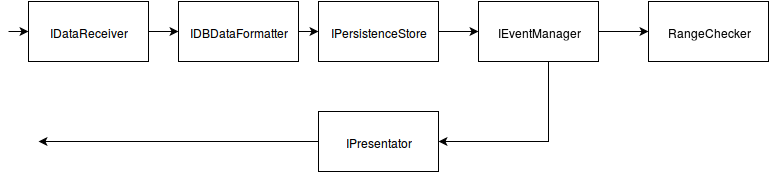
\includegraphics[width=\linewidth]{../../Docs/ProjectReport/Figures/LogicArchitecture/Server/FlowDiagramNewRange.png}
      \caption{New Range Stream}
    \end{figure}
    \begin{figure}
      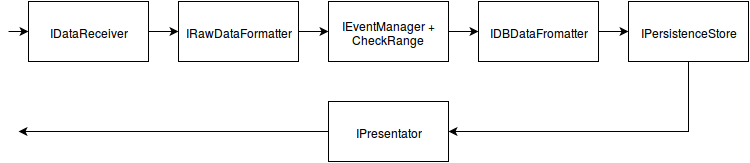
\includegraphics[width=\linewidth]{../../Docs/ProjectReport/Figures/LogicArchitecture/Server/FlowDiagramReceiveData.png}
      \caption{Incoming Data Stream}
    \end{figure}
    \begin{figure}
      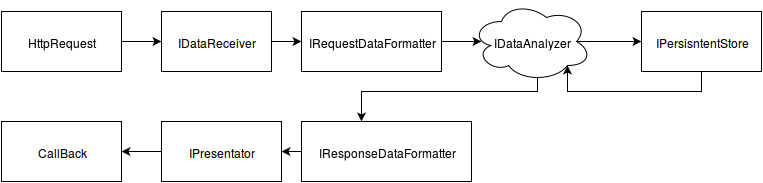
\includegraphics[width=\linewidth]{../../Docs/ProjectReport/Figures/LogicArchitecture/Server/FlowDiagramViewData.png}
      \caption{Request Data Stream}
    \end{figure}
    \column{.5\textwidth} % Right column and width
      \begin{figure}
        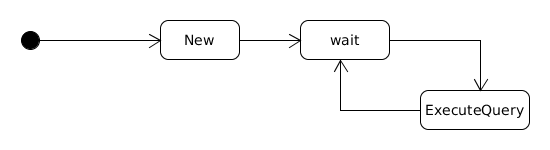
\includegraphics[width=\linewidth]{../../Docs/ProjectReport/Figures/LogicArchitecture/Server/IPersistenceStoreBehavior.png}
        \caption{Persistence Store Behaviour}
      \end{figure}
      \begin{figure}
        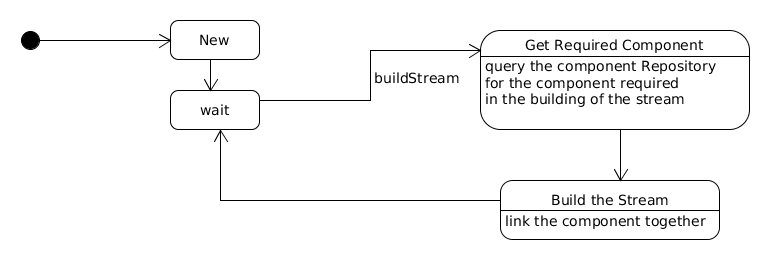
\includegraphics[width=\linewidth]{../../Docs/ProjectReport/Figures/LogicArchitecture/Server/IStreamBuiderBehavior.png}
        \caption{Stream Builder Behaviour}
      \end{figure}
    \end{columns}
\end{frame}

\section{Project}

\subsection{Technologies and Tools}

\begin{frame}
  \frametitle{Technologies and Tools}
        \begin{figure}
        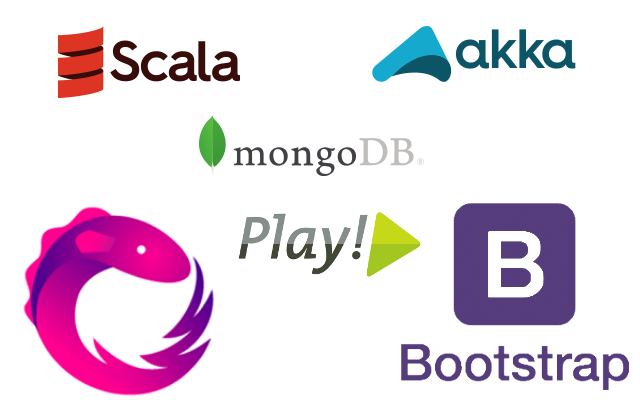
\includegraphics[width=\linewidth]{../../Docs/ProjectReport/Figures/ToolsLogos.png}
        \caption{Stream Builder Behaviour}
      \end{figure}
\end{frame}

\subsection{Project Architecture Differences}

\begin{frame}
  \frametitle{Project Architecture Differences}
  \begin{itemize}
    \item \textit{Web Pages:} vengono utilizzate come output dell'elaborazione, grazie anche al supporto del play framework.
    \item \textit{Startup:} era stata prevista una classe che si occupasse della creazione dei vari elementi del sistema, mentre invece questo viene effettuato dal framework.
    \item \textit{Data Analisys:} per computazioni di analisi sui dati erano stati previsti degli oggetti specifici, mentre, per semplicit\'a si \'e demandato tutto a primitive del DBMS (average, max, min).
    \item \textit{Rappresentazione Interna delle Entit\'a di Dominio:} Per tutte le entit\'a di dominio interne al sistema \'e stata pensata una rappresentazione interna per rendere indipendente il sistema stesso dalle rappresentazioni provenienti dall'esterno e quelle necessarie per il persistence store. Sono state necessarie anche l'implementazione di operazioni di conversione.
  \end{itemize}
\end{frame}

\begin{frame}
\frametitle{References}
\footnotesize{
\begin{thebibliography}{99} % Beamer does not support BibTeX so references must be inserted manually as below
  \bibitem[Reactive Manifesto]{reactiveManifesto} Reactive Manifesto
    \newblock \url{http://www.reactivemanifesto.org/}

  \bibitem[Reactive Extensions]{reactiveExtensions} Reactive Extensions
    \newblock \url{http://reactivex.io/}

  \bibitem[Play Framework]{PlayFramework} Play Framework
    \newblock \url{https://www.playframework.com/}

  \bibitem[Scala Language]{ScalaLanguage} Scala Language
    \newblock \url{http://www.scala-lang.org/}

  \bibitem[MongoDB]{mongoDB} MongoDB
    \newblock \url{https://www.mongodb.org/}


  \bibitem[Akka Framework]{AkkaFramework} Akka Framework
    \newblock \url{http://akka.io/}


  \bibitem[Bootstrap]{bootstrap} Bootstrap
    \newblock \url{http://getbootstrap.com/}

\end{thebibliography}
}
\end{frame}


\end{document} 
